\chapter{图与连接结构}
\label{chap:graph-objects}
\label{chap:graph-paths}

城市之间修了哪些道路，一项工程里哪项任务必须等另一项完成，这类信息都由“有限个对象”和“对象之间的直接连接”组成。我们关心的往往不是某一条连接本身，而是由连接串起来的整体：从一座城市能否开车到达另一座，拆掉一座桥以后交通网会不会断成两片，一组任务能否排出不违反依赖的先后次序。回答这些问题之前，先要说清图记录了什么、没有记录什么。

本章用集合、关系与映射的语言建立图这一对象，并沿“一步连接—多步连接—整体结构”的顺序展开。第~\ref{sec:graph-basic-concepts}节规定图记录哪些连接，方向、边权和子图分别附加或取出什么信息。一步的连接首尾相接，得到第~\ref{sec:graph-adjacency-paths}节的行走、路径与可达关系。无向图中的可达关系是等价关系，第~\ref{sec:graph-connectivity-separation}节据此把顶点划分为连通分量，并考察删除顶点或边怎样切断连接。

切断连接的研究说明，环上的边删去后图仍然连通。所以用最少的边保持连通的结构没有环，这就是第~\ref{sec:graph-trees-forests}节的树：它的路径唯一，边数恰为顶点数减一。最后两节转向记录与比较。第~\ref{sec:graph-representations}节比较四种表示的访问代价，其中邻接矩阵把行走计数变成矩阵乘法；第~\ref{sec:graph-isomorphism}节用同构判断两张图是否只差一套顶点名称。全章用同一张四个顶点、五条边的小图作贯穿例子。

本章只建立定义、基本性质和对给定结果的核对方法，所用的例子都小到可以手工完成。在大图上系统地求出可达集、连通分量、生成树和拓扑次序，需要广度优先遍历与深度优先遍历等算法，这是第~\ref{chap:graph-traversal}章的任务。带权路径的最短成本和总成本最小的生成树，分别在第~\ref{chap:shortest-paths}章和第~\ref{chap:minimum-spanning-tree}章讨论。

\section{图的基本概念}
\label{sec:graph-basic-concepts}

道路网记录哪些城市之间有直达道路，任务清单记录哪项任务直接依赖哪项任务。两者都由有限个对象和对象之间成对的直接连接组成，图就是描述这类信息的数学对象。本节先给出最简单的无向图，再根据实际需要依次加入方向和数值，最后讨论怎样从一张图中取出一部分。

\subsection{图的定义}
\label{sec:graph-conn-definition}

同一张道路网可以画成很多样子：城市的位置可以挪动，道路可以画直或画弯，两条道路在纸上还可能交叉。要判断两幅画描述的是不是同一张网，先得说清哪些内容是数据，哪些只是画法。对于“能否直达”这个问题，数据只有两样：有哪些城市，哪些城市之间有直达道路。

\paragraph{顶点集与边集}
把每个对象记为一个顶点，把每一对有直接连接的对象记为一条边，就得到一张图。这里先考虑没有方向的连接，例如可以双向通行的道路。

\begin{definition}[图]
\label{def:graph-conn-graph}
设$V$是有限集合，$E$是由$V$中两个不同元素组成的无序对$\{i,j\}$的集合，称$\mathcal G=(V,E)$为一个（无向）\term{图}（graph）。$V$中的元素称为\term{顶点}（vertex），$E$中的元素称为\term{边}（edge）。若$\{i,j\}\in E$，称$i,j$是这条边的两个端点。
\end{definition}

记$n=|V|$为顶点数，$m=|E|$为边数。全章使用同一个例子：
\begin{equation}
V=\{1,2,3,4\},\qquad
E=\bigl\{\{1,2\},\{1,3\},\{2,3\},\{2,4\},\{3,4\}\bigr\},
\label{eq:graph-conn-running-graph}
\end{equation}
它有$n=4$个顶点、$m=5$条边，可以看成两个三角形$\{1,2,3\}$与$\{2,3,4\}$共用边$\{2,3\}$。四个顶点之间最多有$\binom42=6$条边，这里只缺$\{1,4\}$。

\paragraph{图相等的判断}
既然图只由$V$和$E$确定，比较两幅图时只需读出各自的顶点集，把每条线段写成由两个端点组成的无序对，再比较两个顶点集和两个边集。图~\ref{fig:graph-conn-running-drawings}的三幅画顶点位置、线段形状和交叉情况都不同，读出的集合却都是式\eqref{eq:graph-conn-running-graph}，因此是同一张图。读边时只看端点，所以画面上的交叉点不是顶点，线段的长短也不是边的长度。问题若需要长度、坐标这样的数值，必须另外给出，见第~\ref{sec:graph-conn-weights}小节。

\begin{figure}[!htb]
  \centering
  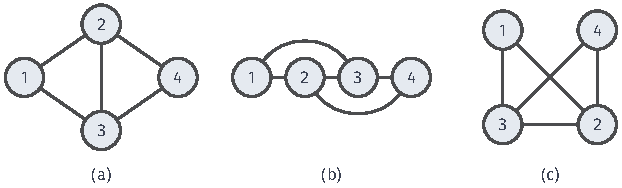
\includegraphics[width=106.765mm]{figures/01-basic-mathematics/04-graphs/tikz/c1-running-graph-drawings/figure.pdf}
  \caption{贯穿全章的四点五边图\eqref{eq:graph-conn-running-graph}的三种画法。顶点位置、线段形状和交叉情况都不同，但边集都是$\{1,2\},\{1,3\},\{2,3\},\{2,4\},\{3,4\}$。(c)中两条对角边在画面上交叉，交叉处不是顶点。}
  \label{fig:graph-conn-running-drawings}
\end{figure}

\paragraph{简单图}
定义~\ref{def:graph-conn-graph}要求边的两个端点不同，并且边集是普通集合，因此排除了一个顶点连到自身的\term{自环}（self-loop），也排除了同一对顶点之间的多条\term{平行边}（parallel edges）。满足这两条限制的图称为\term{简单图}（simple graph），本部分默认讨论有限简单图。简单图的每条边都是$V$的一个二元子集，而$n$元集合的二元子集共有$\binom n2$个，所以$m\leq\binom n2$。

如果两条平行道路需要分别记录收费，就得给每条边一个独立的身份，这时上面的边数上限也不再成立；用到这类扩展时会明确指出。另一个边界情形是顶点集为空的图。它只在少数论证中出现；结论需要至少一个顶点时，我们写明“非空图”。

\subsection{无向图与有向图}
\label{sec:graph-conn-directions}

道路可以双向通行，任务之间的依赖却有先后：“任务$i$完成后才能开始任务$j$”与“任务$j$完成后才能开始任务$i$”是两回事。无序对满足$\{i,j\}=\{j,i\}$，读不出谁在前。把每个依赖写成先做的任务在前的有序对$(i,j)$，次序就成了数据的一部分。

\begin{definition}[有向图]
\label{def:graph-conn-digraph}
设$V$是有限集合，$E\subseteq\{(i,j)\in V\times V:i\neq j\}$，称$\mathcal G=(V,E)$为\term{有向图}（directed graph）。有序对$(i,j)\in E$称为从$i$到$j$的\term{弧}（arc），也记作$i\to j$；$i$是它的起点，$j$是它的终点。
\end{definition}

为了区分，以无序对为边的图也称\term{无向图}（undirected graph）。有向图的弧集仍记作$E$，弧数仍记作$m$。弧$i\to j$只允许从$i$一步到达$j$，并不包含反向的$j\to i$。

图~\ref{fig:graph-conn-edge-vs-arcs}对照了无向边$\{u,v\}$与一对反向弧$(u,v),(v,u)$。两者都允许在$u,v$之间来回，区别在于无向边是一条连接，删除它就同时失去两个方向；两条弧是两个独立的对象，可以只删除其中一条，也可以分别附上不同的数值，例如上坡和下坡的用时。所以用一对反向弧代替每条边来改写无向图时，$m$条边变成了$2m$条弧，边的个数和身份都变了。

\begin{figure}[!htb]
  \centering
  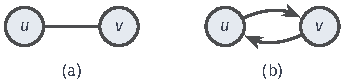
\includegraphics[width=62.974mm]{figures/01-basic-mathematics/04-graphs/tikz/c1-edge-vs-arcs/figure.pdf}
  \caption{一条无向边(a)与一对反向弧(b)都允许在$u,v$之间往返，但(b)中的两条弧是两个独立对象，可以分别删除或另附数值。}
  \label{fig:graph-conn-edge-vs-arcs}
\end{figure}

方向还决定了从哪里能走到哪里。图~\ref{fig:graph-conn-direction-orientation}给同一条三点连接1—2—3赋予不同的方向。不定向时，三个顶点两两可以互相到达；定向为$1\to2\to3$后，从$1$可以经$2$到达$3$，从$3$却哪里也去不了；定向为$1\to2\leftarrow3$后，$1$和$3$都只能到达$2$。

\begin{figure}[!htb]
  \centering
  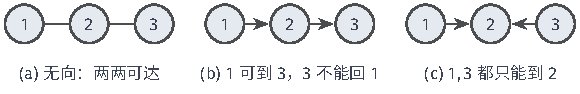
\includegraphics[width=98.189mm]{figures/01-basic-mathematics/04-graphs/tikz/c1-direction-orientation/figure.pdf}
  \caption{同一条三点连接的无向形式(a)与两种定向(b)(c)。箭头决定了从哪个顶点能走到哪个顶点。}
  \label{fig:graph-conn-direction-orientation}
\end{figure}

\paragraph{底层无向图}
有时只关心两个对象之间有没有直接联系，而不在乎谁先谁后。这时把每条弧$(i,j)$改写成无序对$\{i,j\}$放进一个新的边集；$(i,j)$与$(j,i)$同时出现时，集合中只留下一条边。得到的无向图称为原图的\term{底层无向图}（underlying undirected graph）。图~\ref{fig:graph-conn-direction-orientation}中(b)(c)的底层无向图都是(a)。这样做丢掉了先后：(a)中$3$能到达$1$，(b)中却不能，因此不能根据底层无向图断言原来的有向图可以双向到达。第~\ref{sec:graph-connectivity-separation}节定义弱连通时会用到底层无向图。

\subsection{边权与属性}
\label{sec:graph-conn-weights}

许多问题还需要每条连接上的一个数：道路有多长，管道每秒最多输送多少，两个样本有多相似。给定映射$w:E\to\mathbb R$，它在一条边$\{i,j\}$（或弧$(i,j)$）上的值称为\term{边权}（edge weight）；没有边的顶点对没有边权。

同一组边权在不同问题中参与的运算可以完全不同。图~\ref{fig:graph-conn-weight-semantics}在同一边集上附加同一组数，给出三种读法。读作长度$\ell_{i,j}$时，数值沿路线相加，路线$1,2,4$的总长是$2+1=3$，越小越好；读作容量$c_{i,j}$时，数值是单条边的流量上限，边$\{1,3\}$上至多通过$1$个单位，并不沿路线相加；读作相似度$w_{i,j}$时，权重越大，后续计算越强地要求两端的取值接近。所以拿到一张带权图，要先弄清权重的用途。

\begin{figure*}[!htb]
  \centering
  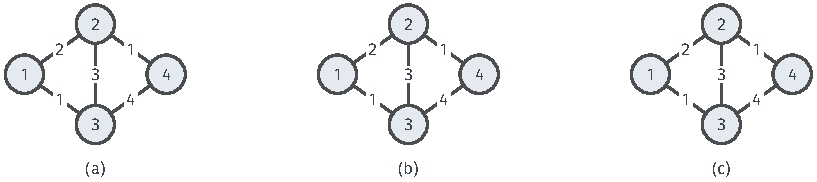
\includegraphics[width=138.187mm]{figures/01-basic-mathematics/04-graphs/tikz/c1-weight-semantics/figure.pdf}
  \caption{同一边集上的同一组边权在三种问题中的读法。(a)长度沿路线相加，路线$1,2,4$的总长为$3$；(b)容量限制单条边的通过量；(c)相似度越大，越要求两端取值接近。}
  \label{fig:graph-conn-weight-semantics}
\end{figure*}

\paragraph{无边与零权边}
边权为$0$不等于没有边。零长度的道路表示免费通行，零容量的管道不能输送正流量，零相似度在加权求和中不贡献数值，但这些边在结构上都还在。图~\ref{fig:graph-conn-zero-weight}中，两种情形在数值记录里都是$0$，只有(b)中顶点$1,2$相邻。能否一步到达要查边集，沿边累计多少才查边权。第~\ref{sec:graph-representations}节用矩阵记录图时，这一区别会变成具体的存储问题。

边权能否为负同样由问题决定，定义本身不作限制。负长度会让“沿路线相加取最小”出现新的困难，第~\ref{chap:shortest-paths}章专门处理；以相似度为权的计算则通常要求权重非负。使用带权图的结论时，要先确认它对边权符号的要求。

\begin{figure}[!htb]
  \centering
  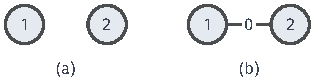
\includegraphics[width=53.188mm]{figures/01-basic-mathematics/04-graphs/tikz/c1-zero-weight-edge/figure.pdf}
  \caption{无边(a)与零权边(b)。二者在数值上都记为$0$，但只有(b)中顶点$1,2$相邻。}
  \label{fig:graph-conn-zero-weight}
\end{figure}

\paragraph{顶点属性与边属性}
边上还可以记录类别、时间等数据，顶点上也可以记录人口、坐标等数据，分别称为边属性和顶点属性。顶点的名称$1,2,3,4$只用来区分顶点，本身不是属性。第~\ref{sec:graph-isomorphism}节会看到，换一套名称不改变图的结构，而属性是否也必须保持，要由问题来规定。

\subsection{子图与诱导子图}
\label{sec:graph-conn-subgraphs}

研究道路网时，我们常常只关心其中一部分城市，或者想知道封闭几条道路以后还剩下什么。取出的部分要仍是一张图，只需保证留下的每条边两个端点都还在。正式地说，若$V'\subseteq V$，$E'\subseteq E$，并且$E'$中每条边的两个端点都在$V'$中，称$\mathcal G'=(V',E')$是$\mathcal G$的\term{子图}（subgraph）。

最常用的两种子图来自删除操作。删除一条边$e$只去掉这条边，记作$\mathcal G-e$；删除一个顶点集$S$则去掉$S$中的顶点，连同所有至少有一个端点在$S$中的边，记作$\mathcal G-S$。删除顶点时必须连带删边，否则留下的边会缺少端点，不再构成子图。

图~\ref{fig:graph-conn-subgraph-induced}(d)只删除了边$\{2,3\}$。(b)(c)保留了同一组顶点$\{1,2,3\}$，边集却不同，可见只给出顶点集合还不能确定一个子图。

\begin{figure*}[!htb]
  \centering
  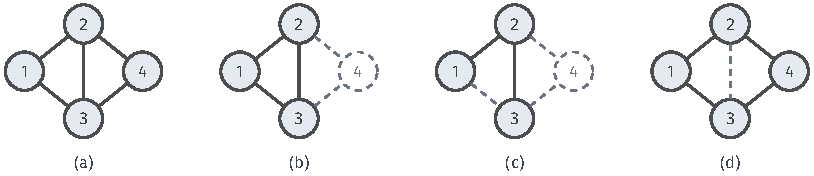
\includegraphics[width=137.686mm]{figures/01-basic-mathematics/04-graphs/tikz/c1-subgraph-induced/figure.pdf}
  \caption{贯穿图的几种子图，灰色虚线表示被删除的顶点或边。(b)删除顶点$4$及其两条边，恰好得到顶点集$\{1,2,3\}$上的诱导子图；(c)保留同样三个顶点，却漏掉了原图中的边$\{1,3\}$，是子图但不是诱导子图；(d)只删除一条边，顶点全部保留。}
  \label{fig:graph-conn-subgraph-induced}
\end{figure*}

\paragraph{诱导子图}
只研究一部分顶点时，通常不希望悄悄改变这些顶点之间的关系，于是把原图中两端都在其中的边全部保留下来。

\begin{definition}[诱导子图]
\label{def:graph-conn-induced-subgraph}
设$S\subseteq V$。以$S$为顶点集、以$\{\{i,j\}\in E:i,j\in S\}$为边集的子图，称为$\mathcal G$在$S$上的\term{诱导子图}（induced subgraph），记作$\mathcal G[S]$。有向图的诱导子图保留两端都在$S$中的全部弧。
\end{definition}

与一般子图不同，诱导子图由顶点集唯一确定。构造$\mathcal G[S]$时，标记$S$中的顶点，再逐条扫描边，两端都有标记的就保留。

对贯穿图取$S=\{1,2,3\}$，保留$\{1,2\},\{1,3\},\{2,3\}$，舍去含$4$的两条边，得到图~\ref{fig:graph-conn-subgraph-induced}(b)。核对一个声称的诱导子图，还要反过来检查原图中两端都在$S$中的边是否一条不漏；图(c)漏掉了$\{1,3\}$，所以不是诱导子图。

删除顶点得到的也是诱导子图。$\mathcal G-S$删去的恰好是至少一端在$S$中的边，留下的恰好是两端都在$V\setminus S$中的边，所以$\mathcal G-S=\mathcal G[V\setminus S]$；例如图(b)既是$\mathcal G[\{1,2,3\}]$，也是$\mathcal G-\{4\}$。第~\ref{sec:graph-connectivity-separation}节讨论删除顶点能否切断连接，第~\ref{chap:graph-traversal}章按分隔集把图分块，用到的都是这两种写法。

\section{邻接与路径}
\label{sec:graph-adjacency-paths}

贯穿图\eqref{eq:graph-conn-running-graph}中顶点$1$和$4$之间没有边，却可以先到$2$或$3$，再到$4$。一步能到谁，由边集直接读出；若干步能到谁，要把边首尾相接。本节从一个顶点的直接邻居出发，把一步的连接延长为行走和路径，由此得到环与可达关系。比较不同路线的总长度是第~\ref{chap:shortest-paths}章的问题，这里只讨论哪些顶点序列允许通行。

\subsection{邻接、邻域与度}
\label{sec:graph-conn-neighborhoods}

站在一座城市，首先要知道哪些城市与它有直达道路，这样的城市有几座。在无向图中，若$\{i,j\}\in E$，称$i$与$j$\term{邻接}（adjacent），互为邻居。顶点$i$的全部邻居组成它的\term{邻域}（neighborhood）
\[
N(i)=\{j\in V:\{i,j\}\in E\},
\]
邻居的个数$d_i=|N(i)|$称为$i$的\term{度}（degree）。

贯穿图中$N(1)=\{2,3\}$，$N(2)=\{1,3,4\}$，四个顶点的度依次为$2,3,3,2$。度只数直接邻居，经两步才能到达的$4$不计入$N(1)$。

在有向的依赖关系中，还要分清“我直接依赖谁”和“谁直接依赖我”：弧$i\to j$对两端的意义不同。因此分别定义出邻域与入邻域
\[
N^+(i)=\{j:(i,j)\in E\},\qquad
N^-(i)=\{j:(j,i)\in E\},
\]
二者的大小$d_i^+$与$d_i^-$分别称为\term{出度}（out-degree）与\term{入度}（in-degree）。图~\ref{fig:graph-conn-neighborhood-degree}在贯穿图和一个小有向图上标出了这些量。

\begin{figure}[!htb]
  \centering
  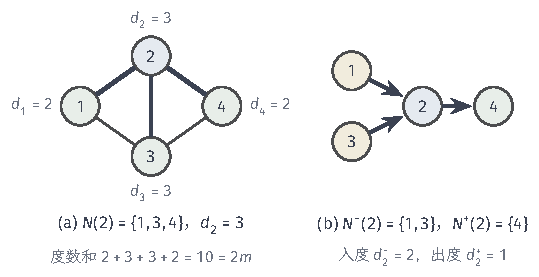
\includegraphics[width=91.271mm]{figures/01-basic-mathematics/04-graphs/tikz/c1-neighborhood-degree/figure.pdf}
  \caption{邻域与度。(a)贯穿图中顶点$2$的邻域$N(2)=\{1,3,4\}$（绿色），连接它们的三条边加粗，所以$d_2=3$；顶点旁标出各点的度，四个度之和$10$恰为边数的两倍。(b)有向图$1\to2$、$3\to2$、$2\to4$中，顶点$2$的入邻域$N^-(2)=\{1,3\}$（黄色）与出邻域$N^+(2)=\{4\}$（绿色），入度为$2$，出度为$1$。}
  \label{fig:graph-conn-neighborhood-degree}
\end{figure}

\paragraph{度数和与边数}
考虑所有“顶点—边”配对$(i,e)$，其中$i$是边$e$的端点。按顶点分组，顶点$i$出现在$d_i$个配对中；按边分组，每条边恰有两个端点。两种分组数的是同一批配对，所以
\begin{equation}
\sum_{i\in V}d_i=2m.
\label{eq:graph-conn-handshake}
\end{equation}
由此可知度为奇数的顶点个数必是偶数。有向图中每条弧恰好贡献一个出度和一个入度，所以$\sum_i d_i^+=\sum_i d_i^-=m$。

\paragraph{邻域与度的读取}
给每个顶点准备一个空的邻居集合和一个初始为$0$的计数器，然后逐条读边：读到$\{i,j\}$时，把$j$放进$N(i)$、$i$放进$N(j)$，两个计数器各加$1$。表~\ref{tab:graph-conn-degree-trace}是贯穿图上计数器的变化。每读一条边，度数和加$2$，读完$m$条边就是$2m$，这正是式\eqref{eq:graph-conn-handshake}；最后一列若不等于两倍边数，说明某条边只记了一端。

有向图读到弧$(i,j)$时，把$j$放进$N^+(i)$、$i$放进$N^-(j)$。图~\ref{fig:graph-conn-direction-orientation}(c)的$1\to2\leftarrow3$读完后$N^-(2)=\{1,3\}$，$N^+(2)=\varnothing$；不说明方向，就可能把入邻居误当成下一步可以到达的顶点。这里的度只数结构上的边；边带权时把一个顶点所有邻边的权相加，得到的是另一个量，本部分不使用。

\begin{table}[!htb]
  \centering
  \caption{逐条读入贯穿图的边时，四个度计数器的变化。每读一条边，恰有两个计数器各加$1$，度数和每次增加$2$。}
  \label{tab:graph-conn-degree-trace}
  \small
  \begin{tabular}{@{}lccccc@{}}
    \toprule
    已读入的边 & $d_1$ & $d_2$ & $d_3$ & $d_4$ & 度数和\\
    \midrule
    初始 & $0$ & $0$ & $0$ & $0$ & $0$\\
    $\{1,2\}$ & $1$ & $1$ & $0$ & $0$ & $2$\\
    $\{1,3\}$ & $2$ & $1$ & $1$ & $0$ & $4$\\
    $\{2,3\}$ & $2$ & $2$ & $2$ & $0$ & $6$\\
    $\{2,4\}$ & $2$ & $3$ & $2$ & $1$ & $8$\\
    $\{3,4\}$ & $2$ & $3$ & $3$ & $2$ & $10$\\
    \bottomrule
  \end{tabular}
\end{table}

\subsection{行走、路径与环}
\label{sec:graph-conn-walks-paths}

走一步就是从当前顶点走到它的一个邻居，走若干步就得到一串相邻两项都邻接的顶点。是否允许重复经过顶点要看用途：计数多步走法时允许重复，一条实际路线通常不允许。

\begin{definition}[行走与路径]
\label{def:graph-conn-walk-path}
设$\mathcal G=(V,E)$是无向图。顶点序列$(v_0,\ldots,v_k)$若对每个$r=1,\ldots,k$都有$\{v_{r-1},v_r\}\in E$，就称为从$v_0$到$v_k$的一条\term{行走}（walk），$k$称为它的长度，即经过的边数。若行走中的顶点两两不同，就称为一条简单\term{路径}（path）。
\end{definition}

单个顶点$(v_0)$是长度为零的行走，也是长度为零的路径。本部分不加修饰的“路径”都指简单路径。

绕一圈回到起点的路线还要与原路折返区分开。首尾相同（$v_0=v_k$）的行走称为\term{闭行走}（closed walk），但闭合不意味着绕成一圈：沿一条边去而复返的$(2,4,2)$是闭行走，却没有提供第二条路线。

因此把长度$k\geq3$、且$v_0,\ldots,v_{k-1}$两两不同的闭行走称为\term{环}（cycle）；长度为$1$的闭行走需要自环，长度为$2$的只能沿同一条边往返，所以要求$k\geq3$。同一个环可以从不同顶点出发、沿两个方向书写，例如$(1,2,3,1)$与$(1,3,2,1)$，我们把经过同一组边的序列看成同一个环。

\paragraph{顶点序列的核对}
判断一个顶点序列属于哪一类，按定义依次检查：每一步$\{v_{r-1},v_r\}$是否为边，判断行走；从左到右维护“已出现顶点”的集合，看有无重复，判断路径；再要求$k\geq3$、首尾相同且前$k$个顶点不重复，判断环。

图~\ref{fig:graph-conn-walk-path-cycle}给出四个结果：$(1,2,3,1,2)$是行走，但第二次读到$1$时重复，不是路径；$(1,2,4)$是路径；$(2,4,2)$是闭行走而不是环；$(1,2,3,1)$是环。

三者逐步加强，反过来都不成立：行走便于拼接与计数，路径对应实际路线，环表示存在替代路线。

\begin{figure*}[!htb]
  \centering
  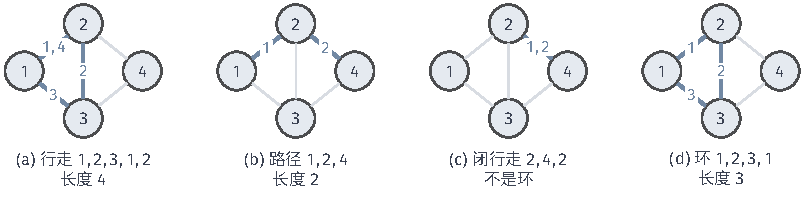
\includegraphics[width=136.186mm]{figures/01-basic-mathematics/04-graphs/tikz/c1-walk-path-cycle/figure.pdf}
  \caption{贯穿图上的四种顶点序列。蓝色粗线是经过的边，边旁数字是经过该边的步序，浅灰色是未经过的边。(a)行走可以重复经过边$\{1,2\}$；(b)路径不重复顶点；(c)沿一条边去而复返得到闭行走，但它不是环；(d)绕三角形一周的环除首尾外不重复顶点。}
  \label{fig:graph-conn-walk-path-cycle}
\end{figure*}

\subsection{有向路径与有向无环图}
\label{sec:graph-conn-dag}

任务依赖要求每一步都顺着箭头走。若顺着箭头走一圈又回到出发的任务，例如$1$等$2$、$2$等$3$、$3$又等$1$，这组任务就无法按任何次序全部完成。把定义~\ref{def:graph-conn-walk-path}中的条件换成$(v_{r-1},v_r)\in E$，就得到有向行走与\term{有向路径}（directed path）。除首尾外顶点两两不同、长度至少为$1$的有向闭行走称为\term{有向环}（directed cycle）；由于没有自环，其长度至少为$2$。

\begin{definition}[有向无环图]
\label{def:graph-conn-dag}
不含有向环的有向图称为\term{有向无环图}（directed acyclic graph，DAG）。
\end{definition}

有向环的最短长度与无向情形不同。图~\ref{fig:graph-conn-directed-cycle-dag}(a)中两条反向弧$i\to j$和$j\to i$是两个不同的对象，$(i,j,i)$构成长度为$2$的有向环；无向图中的$(2,4,2)$两次经过的是同一条边。图(b)的$(1,2,3,1)$每一步都顺着箭头，是长度为$3$的有向环。

\begin{figure}[!htb]
  \centering
  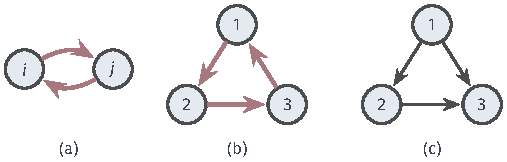
\includegraphics[width=85.937mm]{figures/01-basic-mathematics/04-graphs/tikz/c1-directed-cycle-dag/figure.pdf}
  \caption{有向环与有向无环图。红色弧组成有向环。(a)两条反向弧构成长度为$2$的有向环；(b)三角形的循环定向含有向环；(c)同一个三角形的另一种定向不含有向环，是有向无环图，尽管它的底层无向图是一个环。}
  \label{fig:graph-conn-directed-cycle-dag}
\end{figure}

\paragraph{无环的核对}
有向环上的每个顶点都有环上的弧进出，所以入度或出度为$0$的顶点不在任何有向环上。图~\ref{fig:graph-conn-directed-cycle-dag}(c)的弧为$1\to2$、$1\to3$、$2\to3$，$1$的入度与$3$的出度为$0$，剩下的顶点$2$不足以构成至少含两个顶点的有向环，所以它是DAG。大图上系统地判断有无有向环，要用第~\ref{sec:graph-dfs}节的深度优先遍历或第~\ref{sec:graph-topological-order}节的拓扑排序。

图(c)是DAG，它的底层无向图却是三角形。拓扑排序要求的正是有向无环；换成“底层无向图无环”这一更强的条件，会把(c)这样完全可以排出次序的依赖错误地排除。

\subsection{可达性}
\label{sec:graph-conn-reachability}

很多问题只关心从$i$出发能不能到达$j$，而不关心怎么到。若存在从$i$到$j$的行走，称$j$从$i$\term{可达}（reachable）；有向图中要求有向行走。行走首尾相接仍是行走，路径则未必，所以用行走定义更方便。下面的引理说明改用路径定义并无区别。

\begin{lemma}[行走中含有路径]
\label{lem:graph-conn-walk-contains-path}
在无向图或有向图中，若存在从$i$到$j$的行走，则存在从$i$到$j$的路径，并且它的顶点和边都取自这条行走。
\end{lemma}

\begin{proof}
在从$i$到$j$、顶点和边都取自原行走的所有行走中，取长度最短的一条$(v_0,\ldots,v_k)$。若它不是路径，则有$s<t$使$v_s=v_t$。删去中间段$v_{s+1},\ldots,v_t$，得到$(v_0,\ldots,v_s,v_{t+1},\ldots,v_k)$：原来从$v_t$出发的那一步现在从$v_s=v_t$出发，每一步仍沿原有的边或弧，而长度减少了$t-s>0$，矛盾。
\end{proof}

\paragraph{从行走中取出路径}
实际取出路径时，可以从左到右读一遍行走，随读随删。维护当前路径$P$，初始为$(v_0)$，并给$P$上的顶点做标记。读到$v_r$时，若它没有标记，就接到$P$末尾；若已有标记，说明$P$绕回了$v_r$，就把$P$截到$v_r$所在的位置，并清除其后的标记。$P$始终顶点互异、各边取自原行走，读完时就是所求的路径。每个顶点至多接上、删去各一次，工作量与行走长度成正比。

以行走$(1,2,3,1,3,4)$为例，$P$依次为$(1)$、$(1,2)$、$(1,2,3)$，读到第二个$1$时截回$(1)$，再变为$(1,3)$、$(1,3,4)$。

\paragraph{可达关系的性质}
零长度行走给出自反性，行走首尾相接给出传递性；无向图中把行走倒过来走仍是行走，所以还有对称性。同时满足自反、对称、传递三条的二元关系称为等价关系，所以无向图上的可达关系是等价关系。等价关系的等价类两两不交、并起来恰为全集，下一节据此划分连通分量；等价关系与划分的一般对应，可参考\BookChapterRef{chap:sets-relations-maps}{卷一第~\ref{chap:sets-relations-maps}章}。

这里的性质只说明可达关系是什么。给出两个具体顶点、要判断是否可达，仍需要有组织地访问能走到的顶点，这是第~\ref{sec:graph-bfs}节与第~\ref{sec:graph-dfs}节的任务。

有向图中倒过来走需要反向弧，对称性不再成立：单向链$1\to2\to3$中，$3$从$1$可达，$1$却不从$3$可达。为描述这种单向关系，$N^-(j)$中的顶点称为$j$的直接\term{前驱}（predecessor），$N^+(j)$中的顶点称为直接\term{后继}（successor）；能经一条或多条弧到达$j$的其他顶点称为$j$的\term{祖先}（ancestor），从$j$出发经一条或多条弧能到达的其他顶点称为$j$的\term{后代}（descendant）。本部分约定祖先与后代都不含$j$自身。

单向链中$3$的直接前驱只有$2$，祖先是$\{1,2\}$；$1$的后代是$\{2,3\}$。

有向环上的两个不同顶点可以互为祖先，在DAG中这不可能发生：若$i\neq j$互为祖先，两条有向路径拼成长度至少为$2$的有向闭行走$(v_0,\ldots,v_k)$；在所有满足$s<t$、$v_s=v_t$的位置对中取$t-s$最小的一对，$(v_s,\ldots,v_t)$除首尾外不重复顶点，长度又不能为$1$，所以是有向环，矛盾。可达的不对称使有向图的“连通”需要两种定义，这是下一节的内容。

\section{连通与分隔}
\label{sec:graph-connectivity-separation}

上一节的可达关系一次只回答两个顶点之间的问题。道路网规划还需要整体的回答：全部城市分成几片互相到达的区域，封闭哪些路口或道路会把区域切开。前一个问题由可达关系的等价类回答，有向图中则要区分强、弱两种连通；后一个问题要看删除顶点或边以后是否还有替代路径。这里只讨论结构上的路径是否存在；概率模型中的条件独立另有自己的分离判据，不在本卷讨论。

\subsection{无向图的连通分量}
\label{sec:graph-conn-components}

我们想把全部城市分成若干片，同一片中的城市两两可以互相到达，不同片之间无路可通；有了这样的划分，“能否互相到达”就只需看是否在同一片中。第~\ref{sec:graph-conn-reachability}小节说明，无向图中的可达关系是等价关系；等价类两两不交、并起来恰为$V$，所以它们恰好构成这样的划分。

\begin{definition}[连通分量]
\label{def:graph-conn-component}
无向图$\mathcal G=(V,E)$中可达关系的每个等价类$C\subseteq V$称为$\mathcal G$的一个\term{连通分量}（connected component）；有时也把诱导子图$\mathcal G[C]$称为连通分量。若$\mathcal G$非空且恰有一个连通分量，即任意两个顶点之间都有路径，就称$\mathcal G$是\term{连通}（connected）的。
\end{definition}

这个划分有三条直接的性质。连接同一分量中两点的路径不会离开该分量，因为路径上的每个顶点都与起点可达，所以$\mathcal G[C]$本身连通。不同分量之间没有边，否则两端可达，应属同一分量。划分只取决于可达关系，由图唯一确定。

图~\ref{fig:graph-conn-components}(a)是三角形$\{1,2,3\}$加上孤立顶点$4$，有两个分量$\{1,2,3\}$与$\{4\}$，不连通。空图的分量数为$0$，按定义不算连通，用“恰有一个分量”判断连通时要先排除这个情形。

\begin{figure*}[!htb]
  \centering
  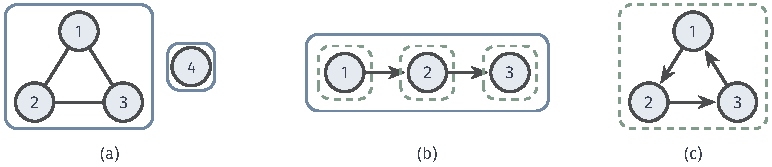
\includegraphics[width=130.652mm]{figures/01-basic-mathematics/04-graphs/tikz/c1-components/figure.pdf}
  \caption{连通分量。蓝色实线框是无向图或底层无向图的连通分量，绿色虚线框是强连通分量。(a)孤立点自成一个分量；(b)单向链$1\to2\to3$忽略方向后连成一片，但没有两个顶点能互相到达，每个顶点自成一个强分量；(c)有向环上任意两个顶点都能互相到达，三个顶点属于同一个强分量。}
  \label{fig:graph-conn-components}
\end{figure*}

\paragraph{分量划分的核对}
核对别人给出的划分不必逐对找路径，上面的前两条性质反过来就够了。

\begin{lemma}[分量划分的核对]
\label{lem:graph-conn-component-check}
设$C_1,\ldots,C_c$是无向图$\mathcal G$的顶点集的一个划分。若每个$\mathcal G[C_k]$都连通，并且没有一条边的两端位于不同的块中，则$C_1,\ldots,C_c$恰好是$\mathcal G$的全部连通分量。
\end{lemma}

\begin{proof}
同一块中的两点由块内连通而可达。反过来，若$j$从$i$可达，取一条行走，它的每一步沿一条边，而没有边跨越不同的块，所以$i,j$在同一块中。于是各块就是可达关系的等价类。
\end{proof}

于是核对分两步：给顶点写上块编号，逐条扫描边，检查两端编号相同；再对每一块给出把块内顶点连在一起的边。图~\ref{fig:graph-conn-components}(a)的划分$(1,1,1,2)$两步都通过；若把贯穿图划分为$\{1,2\}$与$\{3,4\}$，第一步就在边$\{1,3\}$处失败。

第二步所需的块内连接在第~\ref{sec:graph-trees-forests}节整理为生成森林；从零求出全部分量，由第~\ref{sec:graph-connectivity-computation}节在与$n+m$成正比的时间内完成。

一张图是否连通，取决于删去连接以后有没有替代路径。在贯穿图中删除边$\{2,3\}$，$2$与$3$仍可经$1$或$4$相连；在图~\ref{fig:graph-conn-cut-bridge}(a)中删除连接两个三角形的边$\{3,4\}$，图就分成两个分量。两次都只删除一条边，结果不同是因为前者的边位于环上，环的另一侧提供了替代路径。第~\ref{sec:graph-conn-cut-bridge}小节会把这一观察写成桥的判别条件。

\subsection{强连通与弱连通}
\label{sec:graph-conn-strong-weak}

有向图中可达不是等价关系，不能直接用来划分顶点。修补的办法有两种：要求双向都可达，回答哪些顶点能“绕得回来”；或者忽略方向，只问是否连成一片。

若$j$从$i$可达且$i$从$j$可达，称$i,j$相互可达。相互可达关系是自反的（零长度行走）、对称的（定义对$i,j$对称）、传递的（两个方向分别首尾相接），因此是等价关系。它的等价类称为\term{强连通分量}（strongly connected component）；若有向图非空且只有一个强连通分量，就称它\term{强连通}（strongly connected）。

忽略方向的办法用底层无向图（第~\ref{sec:graph-conn-directions}小节）的连通分量划分顶点，所得的分量称为原图的\term{弱连通分量}（weakly connected component）；底层无向图连通时，称原有向图\term{弱连通}（weakly connected）。

在小图上可以直接读出两种分量。记$R^+(v)$与$R^-(v)$分别为从$v$可达与能到达$v$的顶点集（都含$v$），由定义，$v$所在的强分量是
\[
R^+(v)\cap R^-(v);
\]
弱分量则在底层无向图上读出。

图~\ref{fig:graph-conn-components}(b)的单向链中，$R^+(2)=\{2,3\}$，$R^-(2)=\{1,2\}$，所以$2$所在的强分量是
\[
R^+(2)\cap R^-(2)=\{2,3\}\cap\{1,2\}=\{2\}.
\]
同理三个顶点各成一个强分量，却只有一个弱分量。(c)的有向环中两个可达集都是$\{1,2,3\}$，图强连通。在大图上求全部强分量的线性时间方法见第~\ref{sec:graph-connectivity-computation}节。

有向路径去掉箭头后是底层无向图中的路径，所以每个强分量都包含在某个弱分量之内，强连通蕴含弱连通。单向链说明反过来不成立。需要回答“能否往返”时，必须使用强分量。

\subsection{分隔集}
\label{sec:graph-conn-separators}

规划者还关心脆弱性：封闭哪些路口能把两个区域隔开。被封闭的路口不能属于要隔开的两组本身；“隔开”的含义是，删掉这些路口以后，两组之间一条路径也不剩。

\begin{definition}[分隔]
\label{def:graph-conn-separation}
设$A,B,S\subseteq V$两两不相交。若在$\mathcal G-S$中不存在从$A$中顶点到$B$中顶点的路径，就称$S$\term{分隔}（separate）$A$与$B$，称$S$为$A$与$B$之间的一个\term{分隔集}（separator）。
\end{definition}

等价地，$\mathcal G$中从$A$到$B$的每条路径都至少经过$S$中的一个顶点，因为$\mathcal G-S$中的路径就是$\mathcal G$中避开$S$的路径。所以验证一个候选集要考虑全部路径，找到一条被阻断的路径并不够。

核对时却不必列举路径：在$\mathcal G-S$中从$A$出发求出可达集$R$（第~\ref{sec:graph-bfs}节的广度优先遍历允许以一组顶点为起点），$S$分隔$A$与$B$当且仅当$R\cap B=\varnothing$。若$A$与$B$原本位于不同分量，空集就分隔它们。

在图~\ref{fig:graph-conn-separator-sets}中取$A=\{1\}$、$B=\{4\}$。删除$\{2\}$后$R=\{1,3,4\}$，路径$(1,3,4)$仍在，$\{2\}$不是分隔集；删除$\{2,3\}$后$1$的邻居全被删去，$R=\{1\}$，$\{2,3\}$是分隔集。

\begin{figure}[!htb]
  \centering
  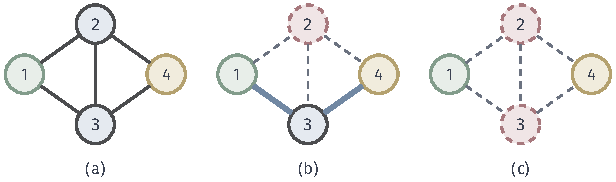
\includegraphics[width=104.186mm]{figures/01-basic-mathematics/04-graphs/tikz/c1-separator-sets/figure.pdf}
  \caption{在贯穿图中检验分隔集，$A=\{1\}$为绿色，$B=\{4\}$为黄色，被删除的候选集$S$为红色虚线顶点。(b)删除$\{2\}$后蓝色路径$(1,3,4)$仍然存在，$\{2\}$不是分隔集；(c)删除$\{2,3\}$后从$1$到$4$没有路径，$\{2,3\}$分隔$\{1\}$与$\{4\}$。}
  \label{fig:graph-conn-separator-sets}
\end{figure}

不指定两组顶点时，分隔集由删除后的分量给出。对连通图$\mathcal G$，若$\mathcal G-S$不连通，则$S$分隔$\mathcal G-S$中任意两个不同分量的顶点集。例如贯穿图删除$\{2,3\}$后余下$\{1\}$与$\{4\}$。第~\ref{sec:graph-separator-blocks}节将沿这样的分隔集把图分成可以分别处理的块。

\subsection{割点与桥}
\label{sec:graph-conn-cut-bridge}

最脆弱的情形是只失去一个路口或一条道路，网络就断开。删除顶点$v$后$\mathcal G-\{v\}$的分量数大于$\mathcal G$的分量数，称$v$为\term{割点}（cut vertex）；删除边$e$后$\mathcal G-e$的分量数大于$\mathcal G$的分量数，称$e$为\term{桥}（bridge）。

图~\ref{fig:graph-conn-cut-bridge}(a)由两个三角形$\{1,2,3\}$、$\{4,5,6\}$和边$\{3,4\}$组成，$3,4$是割点，$\{3,4\}$是桥，三角形内部的边和顶点$1,2,5,6$都不是；(b)的链中，中间顶点$2$是割点，两条边都是桥；(c)的三角形中，删除任意一个顶点或一条边都不会断开。

\begin{figure*}[!htb]
  \centering
  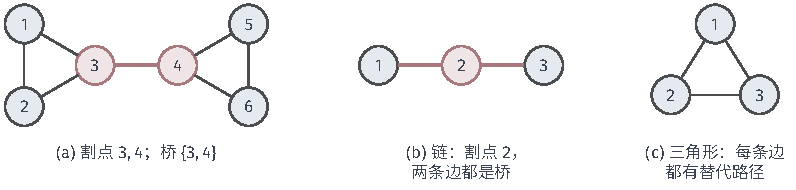
\includegraphics[width=132.687mm]{figures/01-basic-mathematics/04-graphs/tikz/c1-cut-vertex-bridge/figure.pdf}
  \caption{割点与桥，红色顶点为割点，红色粗边为桥。(a)两个三角形由一条边相连，这条边是桥，它的两个端点是割点；(b)链上每条边都是桥，中间顶点是割点，端点$1,3$虽是桥的端点却不是割点；(c)三角形的每条边都位于环上，删除任何一条边或一个顶点都不会断开。}
  \label{fig:graph-conn-cut-bridge}
\end{figure*}

\paragraph{桥的判别}
按定义判断桥要比较删除前后的分量数。下面的定理把它换成只看这条边两端的条件，并说明环正是替代路径的来源。

\begin{theorem}[桥的判别]
\label{thm:graph-conn-bridge-cycle}
设$e=\{i,j\}$是无向图$\mathcal G$的一条边。以下三条等价：(1)$e$是桥；(2)$\mathcal G-e$中没有从$i$到$j$的路径；(3)$e$不在$\mathcal G$的任何环上。并且删除任何一条边，分量数至多增加$1$。
\end{theorem}

\begin{proof}
删除$e$只可能拆开$e$所在的分量$C$。$C$中任一顶点$x$在原图中有到$i$的路径；若它经过$e$，取它第一次到达$i$或$j$之前的部分。这部分不含$e$，所以删除后$x$仍连到$i$或$j$。因此$\mathcal G-e$中$C$至多分成$i$所在和$j$所在两部分，分量数至多增加$1$，并且增加当且仅当$i,j$不再连通，即(1)与(2)等价。

若$e$在某个环上，环的另一侧就是$\mathcal G-e$中从$i$到$j$的路径，所以(2)蕴含(3)；反过来，$\mathcal G-e$中从$i$到$j$的路径长度至少为$2$，接上$e$就是一个环，所以(3)蕴含(2)。
\end{proof}

\paragraph{割点与桥的检验}
由定理，检验$e=\{i,j\}$是否为桥，只需在$\mathcal G-e$中从$i$做一次可达性搜索，看能否到达$j$。例如在图~\ref{fig:graph-conn-cut-bridge}(a)中，删去$\{3,4\}$后从$3$只能到达$\{1,2,3\}$，它是桥；删去$\{1,2\}$后仍可经$3$到达$2$，它不是桥。

检验顶点$v$是否为割点，则删去$v$后从它的一个邻居出发，看能否到达它的其余全部邻居。只看邻居就够了：$v$所在分量中的其他顶点，沿通往$v$的路径走到第一次遇到$v$的邻居为止，这一段避开了$v$，所以它们在删去$v$后仍连到$v$的某个邻居。于是分量是否断开，只取决于$v$的邻居之间是否仍然连通。逐一检验全部顶点或全部边，每次都要做一次这样的搜索。

删点与删边的效果并不对称。删除一个顶点会同时删除它的全部邻边，可能把分量拆成很多块：星形图删除中心顶点后，其余每个顶点都自成一个分量；删除一条边却至多增加一个分量。桥的端点不一定是割点，例如图~\ref{fig:graph-conn-cut-bridge}(b)的端点$1$；没有桥的图也可能有割点，例如两个三角形共用一个顶点。所以“删点能否断开”与“删边能否断开”需要分别检查。

\section{树与森林}
\label{sec:graph-trees-forests}

上一节看到，边位于环上时删掉它不会断开连接，环提供的是冗余的替代路径。若要用尽量少的道路把一组城市连起来，就不应保留任何环。本节研究这种连通而无环的结构。树的两个条件分别对应路径的存在与唯一，由此能数出树的边数，边数又反过来给出判断树的简便方法。

此后两小节讨论树的两种用法：在树上选根可以组织上下层次，在一般连通图中则可以抽出一棵覆盖全部顶点的树。这些结论是第~\ref{chap:graph-traversal}章遍历结果、第~\ref{sec:graph-minimum-spanning-tree}章最小生成树和第~\ref{sec:graph-tree-dp}节树上动态规划的共同基础。

\subsection{树与森林的定义}
\label{sec:graph-conn-tree-definition}

不修多余道路的道路网应当连通，以保证任意两点之间都有路线；还应当无环，因为由定理~\ref{thm:graph-conn-bridge-cycle}，环上的边删去后图仍然连通，可以省掉。同时要求这两点就得到树，只要求无环得到的是若干互不相连的树。

\begin{definition}[树与森林]
\label{def:graph-conn-tree}
非空、连通且不含环的无向图称为\term{树}（tree）。不含环的无向图称为\term{森林}（forest）。
\end{definition}

森林的每个连通分量都连通且无环，是一棵树；只有恰好一个分量的森林才是树。

图~\ref{fig:graph-conn-tree-forest}中，(a)的链和(b)的星形都是树，树可以有分支；(c)的三角形连通但有环，不是树；(d)有三个分量，每个都是树，整体是森林。

两个边界情形需要注意。只有一个顶点、没有边的图是单点树，所以树中的顶点不必都有邻边。空图不含环，是有$0$个分量的空森林，但树要求非空，所以空图不是树。

\begin{figure*}[!htb]
  \centering
  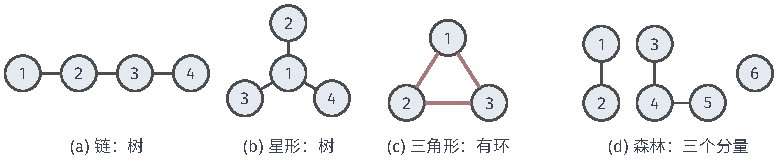
\includegraphics[scale=1]{figures/01-basic-mathematics/04-graphs/tikz/c1-tree-forest/figure.pdf}
  \caption{树、森林与非树的对照。(a)链与(b)星形都是树，后者有分支；(c)三角形连通但含有红色标出的环，不是树；(d)由三个互不相连的树组成的森林，其中孤立顶点$6$是一棵单点树。}
  \label{fig:graph-conn-tree-forest}
\end{figure*}

\subsection{树的基本性质}
\label{sec:graph-conn-tree-properties}

\paragraph{路径唯一性}
树的连通保证任意两点之间有路径，无环则保证这样的路径只有一条。直观上，若两点之间有两条不同的路径，它们分开以后终究要会合，分开与会合之间的两段就围成一个环；反过来，环上相邻的两点既有一条边直接相连，又可以沿环的另一侧到达。

\begin{theorem}[树中路径唯一]
\label{thm:graph-conn-tree-unique-path}
设$\mathcal G$是非空无向图。$\mathcal G$是树，当且仅当任意两个顶点之间恰有一条路径。
\end{theorem}

\begin{proof}
先设$\mathcal G$是树。连通性保证任意两点$u,v$之间至少有一条路径。假设有两条不同的路径$P=(p_0,\ldots,p_a)$与$Q=(q_0,\ldots,q_b)$，$p_0=q_0=u$，$p_a=q_b=v$。一条不能是另一条的真前段，否则较长的那条会两次经过$v$；所以存在最小的$s$使$p_{s+1}\neq q_{s+1}$，记$x=p_s=q_s$。由于$v$同时在两条路径上，可以取$P$在$x$之后第一个也出现在$Q$中$x$之后的顶点$y$。

$P$从$x$到$y$的一段与$Q$从$x$到$y$的一段除端点外没有公共顶点：$P$这一段的中间顶点按$y$的取法不在$Q$中$x$之后的部分，又因为$P$是路径，也不在两者共有的$x$之前的部分。沿$P$从$x$走到$y$，再沿$Q$倒着走回$x$，得到一个除首尾外不重复顶点的闭行走。两段不能都只有一条边，否则$p_{s+1}=y=q_{s+1}$；所以它的长度至少为$3$，是一个环，矛盾。图~\ref{fig:graph-conn-tree-properties}画出了这个构造。

反过来，设任意两点之间恰有一条路径，则$\mathcal G$连通。若$\mathcal G$含环$(c_0,c_1,\ldots,c_{k-1},c_0)$，$k\geq3$，则$(c_0,c_1)$与$(c_0,c_{k-1},\ldots,c_1)$是从$c_0$到$c_1$的两条不同路径，矛盾。
\end{proof}
\begin{BookInlineFigure}
  \centering
  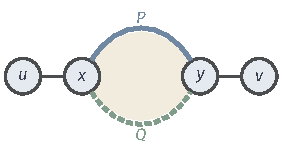
\includegraphics[scale=1]{figures/01-basic-mathematics/04-graphs/tikz/c1-tree-properties/figure.pdf}
  \caption{两条不同路径会围出环。路径$P$（蓝色实线）与$Q$（绿色虚线）在$x$分开、在$y$第一次会合；它们之间的两段构成黄色区域的边界，因此树中不可能同时存在这两条路径。}
  \label{fig:graph-conn-tree-properties}
\end{BookInlineFigure}

由这个定理，删除树的任意一条边$e=\{u,v\}$后$u,v$之间不再有路径，由定理~\ref{thm:graph-conn-bridge-cycle}，树恰好分成两棵较小的树。树的每条边都是桥。

\paragraph{边数}
数树的边数要用到度为$1$的顶点，称为\term{叶}（leaf）。叶只与一个顶点相连，删掉它不会断开其余部分，这使我们能对顶点数归纳。先说明叶总是存在。

\begin{lemma}[树有叶]
\label{lem:graph-conn-tree-leaves}
至少有两个顶点的树至少有两个叶。
\end{lemma}

\begin{proof}
取一条最长的路径$P=(v_0,\ldots,v_k)$，由于树连通且至少有两个顶点，$k\geq1$。若$v_0$另有邻居$z\neq v_1$：$z$不在$P$上时，$(z,v_0,\ldots,v_k)$是更长的路径；$z=v_t$在$P$上时$t\geq2$，$(v_0,v_1,\ldots,v_t,v_0)$是环。两种情形都不可能（图~\ref{fig:graph-conn-tree-properties-leaf}），所以$d_{v_0}=1$。同理$d_{v_k}=1$。
\end{proof}
\begin{BookInlineFigure}
  \centering
  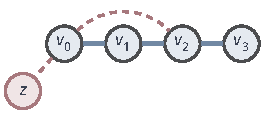
\includegraphics[scale=1]{figures/03-graphs/01-structure-and-computation/tikz/tree-longest-path-leaf/figure.pdf}
  \caption{最长路径的端点必须是叶。若端点$v_0$另有邻居，邻居在路径外（如$z$）会使路径延长，在路径上（如$v_2$）则会形成环；红色虚线表示这两种不可能的连接。}
  \label{fig:graph-conn-tree-properties-leaf}
\end{BookInlineFigure}

\begin{theorem}[树的边数]
\label{thm:graph-conn-tree-edges}
有$n$个顶点的树恰有$n-1$条边。
\end{theorem}

\begin{proof}
对$n$归纳，$n=1$时单点树没有边。设$n\geq2$，由引理~\ref{lem:graph-conn-tree-leaves}，树$\mathcal T$有一个叶$v$。$\mathcal T-\{v\}$无环；它也连通，因为路径的中间顶点要有两条路径上的邻边，度为$1$的$v$不会出现在连接其他两点的路径中间。所以$\mathcal T-\{v\}$是$n-1$个顶点的树，有$n-2$条边，加上$v$的那条边得$n-1$条。
\end{proof}

\subsection{树的判定}
\label{sec:graph-conn-tree-test}

按定义判断一张图是不是树，要确认它没有环，而这是关于全部顶点序列的断言。边数定理提示了另一条途径：数一下边，再查一次连通。为此先说明任何连通图都能用$n-1$条边连成一棵树。

构造从一个顶点出发，每次向外多接一个顶点。任取顶点$r$，令$S=\{r\}$、$F=\varnothing$。只要$S\neq V$，就取$S$外的顶点$t$和一条从$r$到$t$的路径，路径上必有一步从$S$内走到$S$外，把这一步的边加入$F$、它的$S$外端点加入$S$。每一步增加一个顶点和一条边，$n-1$步后$S=V$，$|F|=n-1$。

这样选出的$(V,F)$是树。它连通，因为每个新顶点都连到先前的顶点。它也无环：若$F$中有环，取环上最后加入$S$的顶点$t$，它在环上的两个邻居都更早加入；而$F$中$t$与更早顶点之间的边只有$t$加入时选出的那一条，矛盾。

\begin{theorem}[连通且$n-1$条边的图是树]
\label{thm:graph-conn-connected-tree-test}
设$\mathcal G$是有$n\geq1$个顶点的连通无向图。若$\mathcal G$恰有$n-1$条边，则$\mathcal G$是树。
\end{theorem}

\begin{proof}
按上面的构造选出树$(V,F)$。$F\subseteq E$且$|F|=n-1=|E|$，所以$F=E$。
\end{proof}

\paragraph{森林的边数}
设森林有$n$个顶点、$c$个分量，第$k$个分量有$n_k$个顶点。每个分量是树，有$n_k-1$条边，所以森林的边数是
\begin{equation}
\sum_{k=1}^{c}(n_k-1)=n-c.
\label{eq:graph-conn-spanning-forest-edges}
\end{equation}
于是无环且有$n-1$条边的图只有一个分量，也是树。

\paragraph{三个条件的关系}
对$n\geq1$个顶点的无向图，连通、无环、恰有$n-1$条边三个条件中，前两个由定理~\ref{thm:graph-conn-tree-edges}推出第三个，连通与$n-1$条边由定理~\ref{thm:graph-conn-connected-tree-test}推出无环，无环与$n-1$条边由式\eqref{eq:graph-conn-spanning-forest-edges}推出连通。

只有一个条件不够：三角形加一个孤立顶点（图~\ref{fig:graph-conn-components}(a)）有$4$个顶点、$3$条边，却既不连通又有环。

所以判断树只需两步：若$m\neq n-1$，立即否定；否则查连通。

例如边集为$\{1,2\},\{1,3\},\{1,4\},\{2,5\},\{3,6\}$的六点图有$5=n-1$条边，从$1$出发能到达全部顶点，所以是树；贯穿图有$5\neq3$条边，第一步就被排除。在大图上，第二步由第~\ref{sec:graph-connectivity-computation}节的连通分量计算完成。

\subsection{有根树}
\label{sec:graph-conn-rooted-trees}

家谱、文件目录或分治计算中，每个顶点有一个上级、可能有若干下级，无向树的边却读不出谁是上级。路径唯一性使我们可以从任意一个顶点出发组织这样的层次。

在树$\mathcal T$中选定一个顶点$r$作为根，得到\term{有根树}（rooted tree）。对每个$v\neq r$，从$r$到$v$的唯一路径上紧挨在$v$之前的顶点称为$v$的\term{父节点}（parent），$v$称为它的\term{子节点}（child）。从$r$到$u$的路径经过$v$的那些顶点$u$（包括$v$本身）组成以$v$为根的\term{子树}（subtree）。在有根树中，没有子节点的顶点称为叶。

\paragraph{父子关系的确定}
不必逐个找路径，可以一层层确定：根的邻居都以根为父节点；此后每确定一个顶点$u$的父节点，就把$u$除父节点以外的邻居都定为$u$的子节点。依据是：这样的邻居$w$不在从$r$到$u$的路径上，否则会与边$\{u,w\}$构成环，所以那条路径接上$w$就是从$r$到$w$的唯一路径。

图~\ref{fig:graph-conn-tree-properties-roots}的树有边$\{1,2\},\{1,3\},\{3,4\},\{3,5\}$。以$1$为根时，$2,3$的父节点是$1$，$4,5$的父节点是$3$，叶是$2,4,5$；以$4$为根时，$3$的父节点是$4$，$1,5$的父节点是$3$，$2$的父节点是$1$，叶是$2,5$。根$4$在无向树中是叶，在以它为根的有根树中却不是。第~\ref{chap:graph-traversal}章的遍历在树上给出的就是这样的父子关系。

\begin{BookInlineFigure}
  \centering
  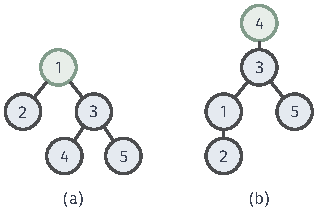
\includegraphics[scale=1]{figures/03-graphs/01-structure-and-computation/tikz/tree-root-choice/figure.pdf}
  \caption{同一棵树的两种选根。(a)以$1$为根，叶是$2,4,5$；(b)以$4$为根，叶是$2,5$。绿色顶点是根，边集不变，父子关系和有根树的叶集合随根改变。}
  \label{fig:graph-conn-tree-properties-roots}
\end{BookInlineFigure}

选根没有增删任何边，只规定每条边上哪一端是父节点；记录$n-1$个非根顶点的父节点就能还原边集，换一个根则全部重新确定。把每条边定向为从父节点指向子节点，得到一张有向图，但这一方向来自选根，而一般有向图的弧方向是原始数据，两者不应混同。第~\ref{sec:graph-tree-dp}节在有根树上自下而上计算时，利用的正是“每个子树只通过它的根与外界相连”。

\subsection{生成树与生成森林}
\label{sec:graph-conn-spanning-trees}

道路网中常要选出一部分道路，使所有城市仍然连通且没有多余的环，例如只维护最少的道路。所选的边必须取自原图，顶点则一个都不能少。

\begin{definition}[生成树与生成森林]
\label{def:graph-conn-spanning-tree}
设$\mathcal G=(V,E)$是无向图。若子图$(V,F)$，$F\subseteq E$，是一棵树，就称它为$\mathcal G$的\term{生成树}（spanning tree）。若$(V,F)$是森林，并且它的连通分量与$\mathcal G$的连通分量相同，就称它为$\mathcal G$的\term{生成森林}（spanning forest）。
\end{definition}

连通图一定有生成树，第~\ref{sec:graph-conn-tree-test}小节的构造选出的$(V,F)$就是一棵；只有连通图才有生成树。在每个分量上各取一棵生成树就得到生成森林，由式\eqref{eq:graph-conn-spanning-forest-edges}，它恰有$n-c$条边，其中$c$是原图的分量数。

\paragraph{生成树的核对与列举}
核对一个声称的生成树，只需检查$F\subseteq E$、$|F|=n-1$、$(V,F)$连通。贯穿图的$T_2$由$\{1,2\},\{1,3\},\{3,4\}$组成，三项都通过；三角形$\{1,2,3\}$的三条边也满足前两项，但没有连到顶点$4$。

同样的判定可以列举全部生成树。从$5$条边中选$3$条共$\binom53=10$种，有环的只有恰好选中三角形$\{1,2,3\}$或$\{2,3,4\}$的两种，所以生成树的个数是
\[
\binom53-2=10-2=8,
\]
见图~\ref{fig:graph-conn-spanning-trees}。

\begin{figure}[!htb]
  \centering
  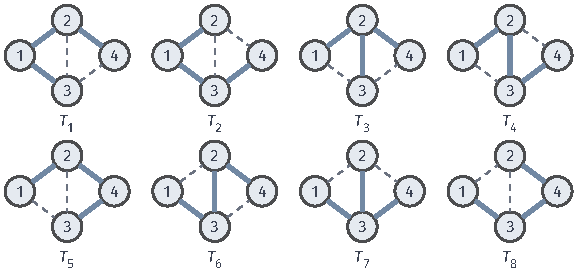
\includegraphics[width=97.652mm]{figures/01-basic-mathematics/04-graphs/tikz/c1-spanning-trees/figure.pdf}
  \caption{贯穿图的全部$8$棵生成树。蓝色粗线是树边，灰色虚线是被舍弃的原边。每棵生成树都有$3$条边并覆盖全部$4$个顶点；从$5$条边中选$3$条的$10$种选法里，只有恰好组成三角形$\{1,2,3\}$或$\{2,3,4\}$的两种不是树。}
  \label{fig:graph-conn-spanning-trees}
\end{figure}

生成树舍弃了环所提供的替代路径。以$T_2$为例：原图中$2,4$相邻，在$T_2$中却要经过$(2,1,3,4)$；原图没有割点，而$T_2$中$1$和$3$都成了割点。所以生成树上的距离和脆弱性一般不等于原图上的结果。生成森林恰好用最少的边给出第~\ref{sec:graph-conn-components}小节核对分量划分所需的块内连接。用遍历求生成森林是第~\ref{sec:graph-connectivity-computation}节的内容，它只保证连通、不比较边权；带建设成本时选总成本最小的一棵，是第~\ref{sec:graph-minimum-spanning-tree}章的问题。

\section{图的表示}
\label{sec:graph-representations}

要让计算机处理一张图，还得决定怎样存储它。不同的算法反复执行的操作不同：有的逐条扫描所有边，有的反复列出一个顶点的邻居，有的查询两个顶点之间是否有边，还有的做矩阵运算。选择记录方式时，要让这些反复执行的操作既正确又便宜。

本节介绍的四种常用表示各为一类操作而设计，图~\ref{fig:graph-conn-four-representations}把贯穿图的四种表示放在一起。比较时既看存储与访问的代价，也计入相互转换的代价；邻接矩阵还把行走计数变成矩阵乘法。代价用记号$O(\cdot)$表示：$O(g)$指操作次数或存储量不超过$g$的某个常数倍，常数与图的规模无关。这一记号描述的是规模增大时的增长速度，增长尺度的比较可参考\BookChapterRef{chap:limits-continuity}{第~\ref{chap:limits-continuity}章}。

\begin{figure}[!htb]
  \centering
  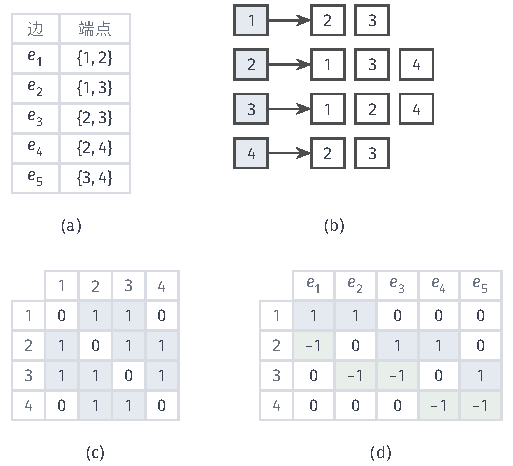
\includegraphics[width=89.524mm]{figures/01-basic-mathematics/04-graphs/tikz/c1-four-representations/figure.pdf}
  \caption{贯穿图的四种表示。(a)边列表逐条记录边的编号和端点；(b)邻接表为每个顶点（蓝色方框）列出邻居，每条无向边在两端各出现一次；(c)邻接矩阵按顶点次序记录每对顶点是否相邻，蓝色为$1$；(d)关联矩阵的每列对应一条边，按“小编号指向大编号”的记录方向，起点处为$1$（蓝色）、终点处为$-1$（绿色）。}
  \label{fig:graph-conn-four-representations}
\end{figure}

\subsection{边列表}
\label{sec:graph-conn-edge-list}

最直接的做法是把边一条条记下来。\term{边表}（edge list），也称边列表，为每条边保存一条记录：边的编号、两个端点，以及长度、容量等所需的属性。有向图的记录必须保存端点的次序。贯穿图的边列表见图~\ref{fig:graph-conn-four-representations}(a)，编号为$e_1=\{1,2\}$、$e_2=\{1,3\}$、$e_3=\{2,3\}$、$e_4=\{2,4\}$、$e_5=\{3,4\}$。有平行边时，两条边端点相同，只能靠编号区分。

边列表除顶点集外只需$O(m)$的存储，适合逐条处理全部边的算法，例如按边权排序（第~\ref{sec:graph-minimum-spanning-tree}章），或每一轮把每条边都检查一遍（第~\ref{sec:graph-shortest-paths}章）；求全部顶点的度也只需扫描一遍，即表~\ref{tab:graph-conn-degree-trace}的做法。它的弱点是查询局部信息：没有额外索引时，列出顶点$2$的邻居或判断$\{1,4\}$是否为边，都要扫描全部$m$条记录。

\subsection{邻接表}
\label{sec:graph-conn-adjacency-list}

遍历一张图时最频繁的操作是“列出当前顶点的全部邻居”，在边列表上每次都要扫描全部记录。\term{邻接表}（adjacency list）预先给每个顶点保存一个列表，列出它的邻居，需要时连同边的属性。无向边$\{i,j\}$在$i$和$j$的列表中各出现一次；有向图的邻接表默认只保存出邻居。

由边列表构造邻接表时，建立$n$个空列表，按编号扫描边列表：遇到无向边$\{i,j\}$，在$i$与$j$的列表末尾各追加对方；遇到弧$(i,j)$，只把$j$追加到$i$的列表。表~\ref{tab:graph-conn-adjacency-list-trace}是贯穿图上的构造过程，最后一行就是图~\ref{fig:graph-conn-four-representations}(b)。建表用$O(n)$时间，每条边追加两次，总共$O(n+m)$。

列表中邻居的次序取决于读边次序，第~\ref{chap:graph-traversal}章的遍历按列表次序读取邻居，所以执行过程会说明采用的次序。有向图若还要列出能一步到达$j$的顶点，就在读到$(i,j)$时再把$i$追加到$j$的入邻居列表，即反向图的出邻居表，存储增加$O(m)$。

\begin{table}[!htb]
  \centering
  \caption{由贯穿图的边列表构造邻接表。每读一条边，在两个端点的列表末尾各追加一项；最后一行即邻接表，各列表的长度依次是度$2,3,3,2$。}
  \label{tab:graph-conn-adjacency-list-trace}
  \small
  \begin{tabular}{@{}lccccc@{}}
    \toprule
    已读入的边 & 顶点$1$ & 顶点$2$ & 顶点$3$ & 顶点$4$ & 列表项总数\\
    \midrule
    初始 & 空 & 空 & 空 & 空 & $0$\\
    $e_1=\{1,2\}$ & $2$ & $1$ & 空 & 空 & $2$\\
    $e_2=\{1,3\}$ & $2,3$ & $1$ & $1$ & 空 & $4$\\
    $e_3=\{2,3\}$ & $2,3$ & $1,3$ & $1,2$ & 空 & $6$\\
    $e_4=\{2,4\}$ & $2,3$ & $1,3,4$ & $1,2$ & $2$ & $8$\\
    $e_5=\{3,4\}$ & $2,3$ & $1,3,4$ & $1,2,4$ & $2,3$ & $10$\\
    \bottomrule
  \end{tabular}
\end{table}

邻接表有$n$个列表头，无向图的列表项共$\sum_i d_i=2m$个（式\eqref{eq:graph-conn-handshake}），有向图的出邻居表共$m$个，所以存储量为$O(n+m)$。列出顶点$i$的邻居只需读它自己的列表，时间与$d_i$成正比；判断$\{i,j\}$是否为边则要在列表中查找，最坏需要$O(d_i)$时间。若一个算法对每个顶点恰好列出一次邻居，总工作量是$\sum_i(1+d_i)=n+2m$；第~\ref{chap:graph-traversal}章正是这样累计遍历的开销。

\subsection{邻接矩阵}
\label{sec:graph-conn-adjacency-matrix}

查询“$i,j$是否相邻”时，邻接表要在列表里查找。若预先给每一对顶点留一个位置，这个查询就能一步完成，代价是更多的存储；把这些位置排成方阵，还能直接使用矩阵运算。

固定顶点次序$1,\ldots,n$。无权图的\term{邻接矩阵}（adjacency matrix）$\bm A\in\mathbb R^{n\times n}$定义为
\begin{equation}
a_{i,j}=
\begin{cases}
1, & \{i,j\}\in E\ \text{（有向图中为}\ (i,j)\in E\text{）},\\
0, & \text{其他情形}.
\end{cases}
\label{eq:graph-conn-adjacency-matrix}
\end{equation}
带权时把有边位置的$1$换成边权$w_{i,j}$，记作$\bm W$。有向图采用“行是起点、列是终点”的约定。无向图的$\bm A$对称，有向图的邻接矩阵一般不对称。

构造时在全零矩阵上逐条填入边：无向边$\{i,j\}$令$a_{i,j}=a_{j,i}=1$，弧$(i,j)$只令$a_{i,j}=1$。贯穿图得到
\begin{equation}
\bm A=
\begin{bmatrix}
0&1&1&0\\
1&0&1&1\\
1&1&0&1\\
0&1&1&0
\end{bmatrix},
\label{eq:graph-conn-running-adjacency}
\end{equation}
第$i$行中为$1$的列号就是$N(i)$，行和就是度$2,3,3,2$，对角元为$0$对应没有自环。

有向图中行和是出度、列和是入度：$1\to2\leftarrow3$的邻接矩阵只有$a_{1,2}=a_{3,2}=1$，第$2$列读出$N^-(2)=\{1,3\}$，第$2$行全为$0$。

\paragraph{零权边与结构掩码}
在权矩阵$\bm W$中，零权边与无边都存成$0$，单看$\bm W$无法区分图~\ref{fig:graph-conn-zero-weight}(a)与(b)。允许零权边时要另存结构掩码$\bm M\in\{0,1\}^{n\times n}$，有边处为$1$。“是否相邻”查$\bm M$，“沿边累计多少”查$\bm W$；使用矩阵的算法应当说明它读的是哪一个。

\paragraph{稠密存储与稀疏存储}
存下全部$n^2$个条目称为稠密存储，查询一对顶点只需$O(1)$时间，列出一个顶点的邻居却要扫描整行，需要$O(n)$时间。

很多实际的图$m$远小于$n^2$：一个有$10^5$个路口的道路网，边数只是几十万量级，稠密邻接矩阵却需要$10^{10}$个条目。稀疏存储只保存非零条目，存储量为$O(n+m)$，按行访问时与邻接表相当。所以说一个算法的代价时必须同时说明存储方式：邻接表上为$O(n+m)$的遍历，搬到稠密矩阵上就变成$O(n^2)$。

\subsection{邻接矩阵的幂与行走计数}
\label{sec:graph-conn-adjacency-powers}

从$1$到$4$走两步有几种走法？走三步回到原处有几种？这类计数在传播过程中反复出现，逐条列举很快变得繁琐。图写成矩阵后，它们可以用矩阵乘法回答；所用的只是乘积的逐项定义$(\bm X\bm Y)_{i,j}=\sum_\ell x_{i,\ell}y_{\ell,j}$，矩阵运算的一般规则可参考\BookChapterRef{chap:linear-operations}{第~\ref{chap:linear-operations}章}。

先看长度为$2$的情形。按乘积的定义，
\[
(\bm A^2)_{i,j}=\sum_{\ell}a_{i,\ell}a_{\ell,j},
\]
而$a_{i,\ell}a_{\ell,j}=1$当且仅当$(i,\ell,j)$是一条长度为$2$的行走。所以对中间顶点$\ell$求和，数出的正是从$i$到$j$长度为$2$的行走条数。这一观察可以推广到任意长度。

\begin{theorem}[邻接矩阵的幂计数行走]
\label{thm:graph-conn-adjacency-powers}
设$\bm A$是无权图（无向或有向）的邻接矩阵，$k\geq0$为整数。则对任意顶点$i,j$，
\begin{equation}
(\bm A^k)_{i,j}=\#\{\text{从}\ i\ \text{到}\ j\ \text{长度为}\ k\ \text{的行走}\}.
\label{eq:graph-conn-adjacency-power-walks}
\end{equation}
\end{theorem}

\begin{proof}
对$k$归纳。$k=0$时$\bm A^0=\bm I$，长度为零的行走只有停在原地的$(i)$。设结论对$k$成立。从$i$到$j$长度为$k+1$的行走按倒数第二个顶点$\ell$分类：它由一条从$i$到$\ell$长度为$k$的行走接上一步$\ell\to j$组成，这一步存在当且仅当$a_{\ell,j}=1$。每条行走恰好落入一类，所以
\[
\#\{\text{从}\ i\ \text{到}\ j\ \text{长度为}\ k+1\ \text{的行走}\}
=\sum_{\ell=1}^{n}(\bm A^k)_{i,\ell}\,a_{\ell,j}
=(\bm A^{k+1})_{i,j}.
\]
\end{proof}

无向图中$(\bm A^2)_{i,j}$就是$i$与$j$的公共邻居个数（$i=j$时是$i$的度）。贯穿图得到
\[
\bm A^2=
\begin{bmatrix}
2&1&1&2\\
1&3&2&1\\
1&2&3&1\\
2&1&1&2
\end{bmatrix}.
\]

图~\ref{fig:graph-conn-adjacency-square}说明了其中第$(1,4)$个条目的来历。按中间顶点求和时只有$\ell=2,3$两项非零，
\[
(\bm A^2)_{1,4}=a_{1,2}a_{2,4}+a_{1,3}a_{3,4}=2,
\]
对应$(1,2,4)$与$(1,3,4)$。对角元$d_i$数的是走到一个邻居再立刻返回的闭行走，它们不是环。

再乘一次$\bm A$可以数三角形。对角元按乘法定义展开为
\[
(\bm A^3)_{i,i}=\sum_j(\bm A^2)_{i,j}a_{j,i},
\]
即对$i$的邻居$j$累加$(\bm A^2)_{i,j}$。贯穿图得对角元$2,4,4,2$，迹为$12$。长度为$3$的闭行走中三个顶点两两相邻，恰好组成一个三角形，而每个三角形可以从$3$个顶点出发、沿$2$个方向绕行，所以三角形个数为
\[
\frac{\operatorname{tr}(\bm A^3)}{6}=\frac{12}{6}=2.
\]

\begin{figure}[!htb]
  \centering
  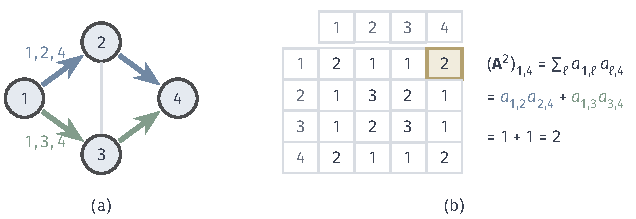
\includegraphics[width=110.352mm]{figures/01-basic-mathematics/04-graphs/tikz/c1-adjacency-square-walks/figure.pdf}
  \caption{邻接矩阵的平方计数长度为$2$的行走。(a)从$1$到$4$的两条行走$(1,2,4)$（蓝色）与$(1,3,4)$（绿色），中间顶点分别是$2$和$3$；(b)贯穿图的$\bm A^2$，黄色条目$(\bm A^2)_{1,4}=2$按中间顶点$\ell$求和，只有$\ell=2,3$的两项非零。}
  \label{fig:graph-conn-adjacency-square}
\end{figure}

\paragraph{计数的范围与代价}
这个计数包含重复顶点的行走，不能直接当作路径数或环数；更长的闭行走会混入往返与重复绕行，不能像三角形那样简单换算。

矩阵幂也能判断可达，但代价很高。由引理~\ref{lem:graph-conn-walk-contains-path}，$j$从$i$可达当且仅当$\bm I+\bm A+\cdots+\bm A^{n-1}$的第$(i,j)$个条目为正，但每次稠密乘法要$n^3$次乘加，远高于遍历的$O(n+m)$；矩阵幂的价值在于计数和代数性质。

带权时$(\bm W^k)_{i,j}$是行走上边权乘积之和，既不是条数也不是长度之和；沿路线相加再取最小，需要把乘法换成加法、求和换成取最小，属于第~\ref{sec:graph-shortest-paths}章。

\subsection{关联矩阵}
\label{sec:graph-conn-incidence-matrix}

邻接矩阵以顶点对为单位，看不出“第几条边”。以边为单位的计算，例如对每条边比较两个端点上的数值，需要行对应顶点、列对应边的矩阵。把边编号为$e_1,\ldots,e_m$，给每条无向边任选一个记录方向，例如把$e_k=\{i,j\}$记为从$i$到$j$。\term{关联矩阵}（incidence matrix）$\bm B\in\mathbb R^{n\times m}$的第$k$列在起点$i$处为$1$、终点$j$处为$-1$，其余为$0$；有向图直接用弧的方向。

构造时按编号读边列表，在第$k$列的起点行写$1$、终点行写$-1$。贯穿图取“小编号指向大编号”的记录方向，得到
\begin{equation}
\bm B=
\begin{bmatrix}
1&1&0&0&0\\
-1&0&1&1&0\\
0&-1&-1&0&1\\
0&0&0&-1&-1
\end{bmatrix},
\label{eq:graph-conn-running-incidence}
\end{equation}
即图~\ref{fig:graph-conn-four-representations}(d)。每列恰有两个非零元且和为$0$，第$i$行的非零元个数等于度$d_i$；不满足这两条的列就是记错的边。

对无向图，记录方向只是一种约定。反转第$k$条边的记录方向，第$k$列整列变号，相当于右乘一个对角元为$\pm1$的对角矩阵，图本身没有改变，所以反映图性质的计算不应依赖这一选择。有向图的弧方向则是数据的一部分。

关联矩阵的列以边为单位，正适合以边为单位的计算。若给每个顶点赋一个数，组成向量$\bm x\in\mathbb R^n$，则$\bm B^{\top}\bm x$的第$k$个分量是
\[
(\bm B^{\top}\bm x)_k=\sum_v b_{v,k}x_v=x_i-x_j,
\]
即第$k$条边记录的起点与终点上数值之差。反转这条边的记录方向只改变差的符号，不改变差的大小。顶点与边上的数值函数、由$\bm B$构造的拉普拉斯矩阵及加权度，可参考\BookChapterRef{chap:graph-functions-operators}{第~\ref{chap:graph-functions-operators}章}。

\subsection{四种表示的比较}
\label{sec:graph-conn-representation-comparison}

表~\ref{tab:graph-conn-representation-costs}汇总了前面各小节的分析。没有一种表示在所有操作上都最好：逐边处理用边列表，逐点列邻居用邻接表，频繁查询顶点对或做矩阵运算用邻接矩阵，以边为单位的线性计算用关联矩阵。

\begin{table}[!htb]
  \centering\small
  \begin{tabular}{@{}lcccc@{}}
    \toprule
    表示 & 存储 & 扫描全部边 & 列出$i$的邻居 & 查询$\{i,j\}$是否为边\\
    \midrule
    边列表 & $O(n+m)$ & $O(m)$ & $O(m)$ & $O(m)$\\
    邻接表 & $O(n+m)$ & $O(n+m)$ & $O(d_i)$ & $O(d_i)$\\
    稠密邻接矩阵 & $O(n^2)$ & $O(n^2)$ & $O(n)$ & $O(1)$\\
    稠密关联矩阵 & $O(nm)$ & $O(nm)$ & $O(m+d_in)$ & $O(m)$\\
    \bottomrule
  \end{tabular}
  \caption{四种表示的存储与三种基本访问的时间代价，$n$为顶点数，$m$为边数，$d_i$为顶点$i$的度。边列表、邻接表不附加索引；稠密关联矩阵列出邻居时先扫描第$i$行找出$d_i$条邻边，再在每条边的列中找另一个端点。关联矩阵若改用按行、按列都可访问的稀疏存储，存储降为$O(n+m)$，列出邻居的代价与邻接表相当。}
  \label{tab:graph-conn-representation-costs}
\end{table}

算法所需的表示往往与输入不同，转换的代价也应计入：边列表与邻接表互转用$O(n+m)$时间；由边列表建稠密邻接矩阵要$O(n^2+m)$，由稠密邻接矩阵建邻接表要读遍$n^2$个条目；建稠密关联矩阵仅置零就要$O(nm)$。

选择表示时，先列出算法反复执行的操作，再按表估计总代价并计入转换与存储：第~\ref{chap:graph-traversal}章的遍历用邻接表，第~\ref{chap:minimum-spanning-tree}章按边权排序用边列表，图上的矩阵算子则用邻接矩阵与关联矩阵。实际程序常同时保存两种表示，额外的存储也应计入。

\section{图同构}
\label{sec:graph-isomorphism}

顶点的名称只是为了区分顶点而取的。把贯穿图的顶点换一套编号，边集的写法会变，邻接矩阵的行列也会移动，连接结构本身却没有变。本节用保持邻接的一一对应把“只差一套名称”写成同构的定义。

有了定义，给定的对应容易核对，不同构也常能用简单的量排除，难的是在没有给出对应时断定同构。最后一小节用置换矩阵把重编号写成矩阵运算。系统比较两张图结构的算法是第~\ref{sec:graph-wl-refinement}节的内容。

\subsection{图同构的定义}
\label{sec:graph-conn-isomorphism-definition}

图~\ref{fig:graph-conn-isomorphism}(a)是贯穿图$\mathcal G$；(c)的$\mathcal G'$顶点集也是$\{1,2,3,4\}$，边集由$\{1,3\}$、$\{1,4\}$、$\{2,3\}$、$\{2,4\}$、$\{3,4\}$组成，两者的边集不相等。但若按(b)的规则$\rho$把$\mathcal G$的顶点改名，$\mathcal G$的五条边依次变为下面五个无序对：
\[
\begin{gathered}
\{1,2\}\mapsto\{1,3\},\qquad
\{1,3\}\mapsto\{1,4\},\qquad
\{2,3\}\mapsto\{3,4\},\\
\{2,4\}\mapsto\{3,2\},\qquad
\{3,4\}\mapsto\{4,2\}.
\end{gathered}
\]
它们恰好是$\mathcal G'$的全部边；唯一不相邻的一对$\{1,4\}$变为$\{1,2\}$，在$\mathcal G'$中也不相邻。可见这样的改名要一一对应，并且相邻的仍相邻，不相邻的仍不相邻。

\begin{figure}[!htb]
  \centering
  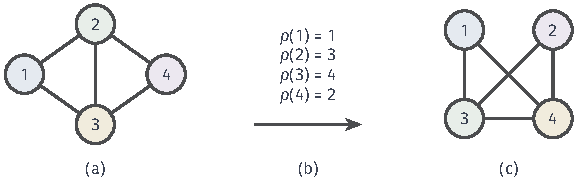
\includegraphics[width=97.688mm]{figures/01-basic-mathematics/04-graphs/tikz/c1-isomorphism-relabeling/figure.pdf}
  \caption{两张同构的图。(a)贯穿图$\mathcal G$；(c)画法与编号都不同的$\mathcal G'$；(b)顶点对应$\rho$。同色顶点互相对应：$\mathcal G$中顶点$i$与$\mathcal G'$中顶点$\rho(i)$颜色相同。逐条核对可见，$\mathcal G$中相邻的顶点对恰好对应$\mathcal G'$中相邻的顶点对。}
  \label{fig:graph-conn-isomorphism}
\end{figure}

\begin{definition}[图同构]
\label{def:graph-conn-isomorphism}
设$\mathcal G=(V,E)$与$\mathcal G'=(V',E')$是无向图。若存在双射$\rho:V\to V'$，使对任意$i,j\in V$都有
\[
\{i,j\}\in E\iff\{\rho(i),\rho(j)\}\in E',
\]
就称$\mathcal G$与$\mathcal G'$\term{同构}（isomorphic），称$\rho$为一个同构映射。
\end{definition}

双向条件不能减弱为单向：边集为$\{1,2\},\{2,3\}$的路径按恒等映射放进三角形$\{1,2,3\}$，边都映为边，但三角形多出了边$\{1,3\}$。反方向的条件保证$\mathcal G'$中不出现多余的连接。

有向图的同构要求$(i,j)\in E\iff(\rho(i),\rho(j))\in E'$。$1\to2\to3$与$1\to2\leftarrow3$的底层无向图相同，作为有向图却不同构：同构映射保持入度，而后者的顶点$2$入度为$2$。加权图还要求$w'_{\rho(i),\rho(j)}=w_{i,j}$；带属性的图要由问题声明哪些属性必须保持，例如顶点带有类别时，可以要求同构映射只把顶点映到同类顶点。

\subsection{同构的核对与排除}
\label{sec:graph-conn-isomorphism-checking}

若别人给出了一个对应$\rho$，只需核对它是否满足定义；若只给出两张图，则要判断是否存在这样的对应，后者困难得多。

\paragraph{给定对应的核对}
定义的条件要对全部$\binom n2$个顶点对检查。下面的引理说明，只需检查边的像，再比较边数。

\begin{lemma}[同构映射的核对]
\label{lem:graph-conn-isomorphism-check}
设$\rho:V\to V'$是双射，$|E|=|E'|$，并且$\mathcal G$的每条边$\{i,j\}$都满足$\{\rho(i),\rho(j)\}\in E'$。则$\rho$是$\mathcal G$到$\mathcal G'$的同构映射。
\end{lemma}

\begin{proof}
由于$\rho$是单射，$\{i,j\}\mapsto\{\rho(i),\rho(j)\}$是从$E$到$E'$的单射；两个有限集合元素个数相同，所以它是双射。于是若$\{\rho(i),\rho(j)\}\in E'$，它是某条边$\{i',j'\}\in E$的像，由$\rho$单射得$\{i',j'\}=\{i,j\}\in E$。
\end{proof}

本节开头的例子正是这样核对的：$\rho$是双射，两图都有$5$条边，五条边的像都在$E'$中，所以$\rho$是同构映射，“不相邻的一对仍不相邻”这一步可以省去。$\mathcal G'$以邻接矩阵存储时，核对用$O(n+m)$时间。

\paragraph{图不变量}
同构映射保持一切由连接结构定义的量：顶点数、边数、每个顶点的度（$\rho$把$i$的邻居一一映为$\rho(i)$的邻居）、度的多重集合、连通分量个数、三角形个数等。这些量称为\term{图不变量}（graph invariant），只要有一个不同，两张图就不同构；计算时宜从便宜的顶点数、边数和排序后的度开始。

例如，六个顶点排成的环与两个互不相连的三角形，顶点数、边数都是$6$，每个顶点的度都是$2$，但前者连通、后者有两个分量，所以不同构。

反过来，比较过的不变量都相同，也不足以断定同构。考虑两棵六个顶点的树，边集分别为
\[
\bigl\{\{1,2\},\{1,3\},\{1,4\},\{2,5\},\{3,6\}\bigr\}
\quad\text{与}\quad
\bigl\{\{1,2\},\{1,3\},\{1,4\},\{2,5\},\{5,6\}\bigr\}.
\]
二者都连通、没有三角形，度的多重集合都是$\{3,2,2,1,1,1\}$。但前一棵树中度为$3$的顶点$1$与两个度为$2$的顶点$2,3$相邻，后一棵树中顶点$1$只与一个度为$2$的顶点$2$相邻。同构映射必须保持度为$3$的顶点及其邻居的度，所以两棵树不同构：比较“邻居的度”能区分只看度区分不了的图。

要得出“同构”的肯定结论，必须真的找到一个对应。逐个尝试全部$n!$个双射再逐个核对，虽然总能判定，但$n=20$时$n!$已超过$2\times10^{18}$。不变量可以缩小搜索，例如度为$3$的顶点只能映到度为$3$的顶点。第~\ref{sec:graph-wl-refinement}节的顶点标记细化把“比较邻居的度”反复执行，并会说明它仍然不能区分所有不同构的图。

\subsection{重编号与置换表示}
\label{sec:graph-conn-relabeling}

当两张图的顶点集都是$\{1,\ldots,n\}$时，同构映射$\rho$就是一个重编号。重编号以后，邻接矩阵的行和列都要按同样的方式重排，置换矩阵恰好执行这种重排，于是同构可以直接在矩阵上核对。

记$\bm e_i$为第$i$个分量为$1$、其余分量为$0$的标准基向量。取置换矩阵$\bm P=\begin{bmatrix}\bm e_{\rho(1)}&\cdots&\bm e_{\rho(n)}\end{bmatrix}$，即第$i$列是$\bm e_{\rho(i)}$，它满足$\bm P\bm e_i=\bm e_{\rho(i)}$。按条目写，$p_{k,i}=1$当且仅当$k=\rho(i)$，其余条目为$0$；由于$\rho$是双射，$\bm P$的每行、每列都恰有一个$1$。

计算$\bm P\bm A\bm P^{\top}$的条目时，按乘法定义展开
\[
(\bm P\bm A\bm P^{\top})_{k,l}=\sum_{i=1}^{n}\sum_{j=1}^{n}p_{k,i}\,a_{i,j}\,p_{l,j}.
\]
求和中只有$k=\rho(i)$且$l=\rho(j)$的一项非零，所以左乘$\bm P$把第$i$行移到第$\rho(i)$行，右乘$\bm P^{\top}$把第$j$列移到第$\rho(j)$列。两者合起来，
\begin{equation}
\bm A'=\bm P\bm A\bm P^{\top},\qquad
a'_{\rho(i),\rho(j)}=a_{i,j}.
\label{eq:graph-conn-relabel}
\end{equation}
原来记录“$i,j$是否相邻”的条目被搬到了新编号的位置。因此，$\rho$是$\mathcal G$到$\mathcal G'$的同构映射，当且仅当$\mathcal G'$的邻接矩阵等于$\bm P\bm A\bm P^{\top}$。

对图~\ref{fig:graph-conn-isomorphism}的$\rho$，$\bm P$的各列依次为$\bm e_1,\bm e_3,\bm e_4,\bm e_2$，即
\[
\bm P=
\begin{bmatrix}
1&0&0&0\\
0&0&0&1\\
0&1&0&0\\
0&0&1&0
\end{bmatrix}.
\]
再取式\eqref{eq:graph-conn-running-adjacency}的$\bm A$，计算得
\[
\bm P\bm A\bm P^{\top}=
\begin{bmatrix}
0&0&1&1\\
0&0&1&1\\
1&1&0&1\\
1&1&1&0
\end{bmatrix}.
\]
这个矩阵的第$1$行读出$N'(1)=\{3,4\}$，第$4$行读出$N'(4)=\{1,2,3\}$，各行都与$\mathcal G'$的边集一致；例如$a'_{3,2}=a'_{\rho(2),\rho(4)}=a_{2,4}=1$。

实际计算不必做矩阵乘法，按第二式把每个条目搬到$(\rho(i),\rho(j))$即可，代价为$O(n^2)$。加权图同样要求$\bm W'=\bm P\bm W\bm P^{\top}$；允许零权边时还要检验结构掩码$\bm M'=\bm P\bm M\bm P^{\top}$。

\paragraph{置换与一般换基}
$\bm P$的各列是互不相同的标准基向量，所以$\bm P^{\top}\bm P=\bm I$，即$\bm P^{\top}=\bm P^{-1}$。于是式\eqref{eq:graph-conn-relabel}可以写成$\bm A'=\bm P\bm A\bm P^{-1}$，是一个相似变换，即在另一组基下表示同一个线性映射（可参考\BookChapterRef{chap:linear-representation}{第~\ref{chap:linear-representation}章}）。

但反过来，一般的相似变换不能都解释为重编号。对两个顶点一条边的图，$\bm A=\left[\begin{smallmatrix}0&1\\1&0\end{smallmatrix}\right]$，取$\bm S=\left[\begin{smallmatrix}1&1\\0&1\end{smallmatrix}\right]$，其逆为$\bm S^{-1}=\left[\begin{smallmatrix}1&-1\\0&1\end{smallmatrix}\right]$。先左乘$\bm S$，
\[
\bm S\bm A
=\begin{bmatrix}1&1\\0&1\end{bmatrix}
\begin{bmatrix}0&1\\1&0\end{bmatrix}
=\begin{bmatrix}1&1\\1&0\end{bmatrix};
\]
再右乘$\bm S^{-1}$，得到
\[
\bm S\bm A\bm S^{-1}
=\begin{bmatrix}1&1\\1&0\end{bmatrix}
\begin{bmatrix}1&-1\\0&1\end{bmatrix}
=\begin{bmatrix}1&0\\1&-1\end{bmatrix}.
\]
这个矩阵不对称，有非零对角元和负条目，不是任何简单无向图的邻接矩阵。一般换基混合不同顶点的坐标，重编号只搬动位置。

相似变换保持特征值，所以邻接矩阵的特征值也是图不变量：特征值不同的两张图一定不同构。但它和其他不变量一样只能排除同构，特征值相同的两张图未必同构。

\section{本章小结}
\label{sec:graph-objects-summary}

本章开头问：图记录了什么，沿连接能到哪里，删除连接会怎样，结构又怎样记录和比较。第一个问题的回答是，图$\mathcal G=(V,E)$只记录有限个对象之间的直接连接，与纸上的画法无关，比较两幅画只需比较顶点集与边集。方向、边权和属性各自附加一类信息。方向决定哪些顶点序列可以通行，忽略方向得到的底层无向图丢掉了先后。边权的含义由问题决定：长度沿路线相加，容量限制单条边的通过量，相似度鼓励两端接近；零权边仍是边，“能否到达”查边集，“累计多少”查边权。子图可以任意保留一部分边，诱导子图则保留选定顶点之间的全部边，因而由顶点集唯一确定。

沿连接能到哪里，由行走和路径回答。行走允许重复，便于拼接与计数；路径不重复顶点，对应实际路线。任何行走都可以随读随删地化成一条同端点的路径，所以用两者定义的可达关系相同。无向图中可达关系是等价关系，它把顶点集唯一地划分为连通分量；核对一个声称的划分，只需检查没有边跨越不同的块、每块内部连通。有向图中可达不对称，要区分要求双向到达的强连通与忽略方向的弱连通，前者蕴含后者，反之不然。任务能否排出先后，取决于有没有顺着箭头绕回起点的有向环；不含有向环的有向无环图，底层无向图仍可以有环。

删除连接的影响由分隔集、割点和桥刻画，判断的依据始终是有没有替代路径。核对分隔集，就是在删除后的图中求出可达集；一条边是桥当且仅当它不在任何环上，删边至多使分量数增加一，删点却可能把分量拆成许多块。用最少的边保持连通，就得到树：树等价于任意两点之间路径唯一，$n$个顶点的树恰有$n-1$条边。连通、无环、恰有$n-1$条边三个条件中任意两个推出第三个，所以判断树只需数边再查连通。选根把树组织成父子层次而不改变边集；生成森林在每个分量上保留一棵生成树，恰有$n-c$条边，并且一般不唯一，它丢掉了原图的替代路径。

同一张图可以用边列表、邻接表、邻接矩阵和关联矩阵记录。四者保存的连接相同，支持的访问和代价不同，转换本身也有代价，选择时应先列出算法反复执行的操作。邻接矩阵还把组合计数变成矩阵运算：$\bm A^k$的条目计数长度为$k$的行走，其中包含重复顶点，不能直接当作路径数。

同构用保持邻接与不相邻的双射刻画“只差一套名称”，在矩阵上表现为置换共轭$\bm A'=\bm P\bm A\bm P^{\top}$。给定对应时，核对边的像并比较边数就够了。度、分量数、特征值等不变量可以排除同构，却不足以确认同构，而逐个尝试$n!$个对应并不可行。

本章说明了怎样在小图上核对连通分量、强连通分量、生成树、无环性和同构，却还没有给出在大图上高效求出它们的方法。第~\ref{chap:graph-traversal}章在邻接表上用广度优先和深度优先遍历实际计算这些对象，用拓扑排序安排有向无环图的次序，并用顶点标记细化比较图的结构；那里的算法输出，仍要按本章的定义与核对方法检验。

